\chapter{Evaluation}\label{ch:evaluation}
Um die Effektivität und Funktion des \cdns zu evaluieren wurden simulierte tests so wie tests unter echten Bedingungen durchgeführt. Neben der Betrachtung der Effektivität ist es ebenfalls wichtig sicherzustellen, das das \cdn von den Nutzern verwendet werden kann dazu wurden die verwendet Browser der Nutzer evaluiert und betrachtet wie viele Nutzer einen geeigneten Browser verwenden. Da die Internetanbindung an Schulen in vielen Fällen nicht gegeben ist wird erläutert wie eine reine Offline Nutzung des \cdns gewährleistet werden könnte. Eine Betrachtung der Implikationen für die Sicherheit bei der Verwendung des \cdns befindet sich am Ende des Kapitels.   
\section{Browser compatbility}
\begin{table}[!htb]
\begin{center}

	\begin{tabular}{|l|l|l|l|l|}
		\hline
		Chrome & Firefox & Edge & Safari & Internet Explorer	  \\ \hline
		22 	   & 23 	  & 76	 & 11	  & Not supported    				\\ \hline
	\end{tabular}
	
	\begin{tabular}{|l|l|l|l|l|}
		\hline
		IOS Safari & Samsung Internet & Android Browser	& Chrome (Android) \\ \hline
		11	   & 4				  & 67				& 76  \\ \hline
	\end{tabular}

	\caption{Unterstützte Browser Versionen}
\end{center}
\end{table}

Um die unterstützten Browser zu verifizieren wurden die vom \pTp \cdn verwendeten Browser Funktionalitäten bei caniuse.com\footnote{https://caniuse.com/} eingegeben. Darüber hinaus wurden Chrome, Firefox, Edge, Safari und der Internet Explorer manuell getestet, um sicherzustellen das das \pTp \cdn das Nutzererlebnis nicht negativ beeinflusst. Der Internet Explorer unterstütz auch in der aktuellen Version keine Service Worker\footnote{https://caniuse.com/#search=service\%20worker}. Auch wenn der Edge Browser Webrtc seit Version 17 unterstützt, ist es leider erst ab version 76 möglich Datachannels zu verwenden. Da der Datenverkehr des \pTp \cdns über Datachannel gehandhabt wird, ist eine Verwendung erst ab der nächsten Version die auf Chrome aufbauen wird, möglich.

\subsection{Browser Nutzung von SlideSync Kunden}

\begin{table}[!htb]\label{table-browser-slidesync}
\begin{center}

	\begin{tabular}{|r|l|l|l|l|l|l|}
		\hline
		Event	 & Intern 	& Extern 	& Unterstützt & Nicht unterstützt \\ \hline
		Event 1	 & 2816		& 4073	  	& 4357		  & 2532		\\ \hline 
		Event 2	 & 50		& 48		 	& 37			  & 60		\\ \hline 
		Event 3	 & 43		& 248	  	& 224		  & 67		\\ \hline 
		Event 4	 & 740		& 569	  	& 735		  & 573		\\ \hline 
		Event 5	 & 300		& 520	  	& 600		  & 220		\\ \hline 
		Event 6	 & 365		& 656	  	& 773		  & 248		\\ \hline 
		Gesamt	 & 4314		& 6114	  	& 6726		  & 3700		\\ \hline 

	\end{tabular}
	\caption{Vergleich von 6 Events}
\end{center}

\end{table}

Um die Browser Nutzung von SlideSync Nutzern zu evaluieren wurden je drei Events von 2 großen Kunden betrachtet. Beide Kunden verwenden momentan einen von SlideSync vertriebenen Netzwerk internen Caching Servern und mit beiden Kunden wird derzeit eine Verwendung des \pTp \cdns anstelle der momentanen \cdn Server diskutiert. Event eins bis drei wurden von Kunden 1 und Event 4 bis 6 wurden von Kunde 2 durchgeführt. 

 Von den insgesamt 10426 betrachteten Browser Sitzungen verfügten 64,5\% über einen Browser der von dem \pTp \cdn unterstützt wird. Die vergleichsweise geringe Prozentzahl ist vor allem auf die nach wie vor starke Verbreitung des Internet Explorers in Unternehmen zurückzuführen. So handelte es sich bei 96,5\% der nicht unterstützen Browser von Event 1 um Nutzer mit Internet Explorer 11. In Gesprächen mit Kunden wurde deutlich das diese jedoch in absehbarer Zeit auf Edge 76 wechseln werden, welcher auf Chrome basiert und damit volle Unterstützung des \cdns bietet.\cite{edge-chrome} Ein Mitarbeiter einer großen Bank gab einen Zeithorizont von ein bis zwei Jahren an. Außerdem würden sie als Bank Updates eher hinauszögern weshalb bei anderen Unternehmen ein kürzerer Zeithorizont zu erwarten wäre.

%tk 2444
%Annual General Meeting 2019
%https://slidesync.com/admin/events/21BNZWjB3y/overview
%Supported	4357
%un sup	2532
%External	4073
%Internal	2816
%https://slidesync.com/admin/events/eavm3EYAMY/statistics
%LEX Global Town Hall Call
%sup	37
%unsup	60
%Internal	50
%External	48
%https://slidesync.com/admin/events/oKkY3x4BwQ/statistics
%Sup	224
%un sup	67
%External	248
%Internal	43
%%Bundesbank:
%%https://slidesync.com/admin/events/ajAZ3VEk2O/statistics
%
%Pro 7
%https://slidesync.com/admin/events/1Oxv7loBlo/statistics
%Sup	735
%no sup	573
%Internal	740
%External	569
%https://slidesync.com/admin/events/rlB6xP6kWR/statistics
%Sup	600
%un sup	220
%External	520
%Internal	300
%https://slidesync.com/admin/events/MwBwGloBEL/statistics
%Sup	600
%un sup	220
%Extern	656
%Intern	365
%öffentlich (landing page)
%Chrome
%607	48,76 %
%2.	
%Internet Explorer
%170	13,65 %
%3.	
%Safari
%156	12,53 %
%4.	
%Firefox
%119	9,56 %
%5.	
%Edge
%58	4,66 %
%6.	
%UC Browser
%56	4,50 %
%7.	
%'Mozilla
%40	3,21 %
%8.	
%Samsung Internet
%15	1,20 %
%\begin{itemize}
%	\item Statistic über typische nutzung
%	\item Statistic über Nutzung bei dem test
%	\item Diskussion Edge on Chromium
%	\item evtl aussage von deutscher bank mit aufnehmen
%	\item  --- major update hinauszögern, in 1-2 Jahren
%	\item Anderer Kunde wechsel kein Problem
%	\item \cite{edge-chrome}
%\end{itemize}


\subsection{Browser usage in eduational networks}
\begin{itemize}
	\item evtl einfach normale verteilung
	\item schauen ob es quellen gibt
\end{itemize}
%\section{Webrtc Routing}
%\begin{itemize}
%	\item mit und ohne STUN
%	\item lokales routing
%	\item externes Routing
%	\item implikationen für Konfiguration
%\end{itemize}
%\section{Bandwidth}


%
%\subsection{Latency}



\section{Simulierter Workload}

Im Folgenden werden verschiedene Tests zur Evaluation des \pTp \cdns vorgestellt und erläutert. Um zu Untersuchen wie sich das \cdn unter verschiedenen Bedingungen verhält wurde die Ladezeit verschieden großer Dateien gemessen, livestreams mit simulierten Nutzern getestet und eine Schulklasse simuliert. Um möglichst viele Variablen kontrollieren zu können wurden die Tests unter Laborbedingungen durchgeführt und alle Nutzer simuliert.

\subsection{Ladezeiten von verschiedenen Dateigrößen}
\begin{figure}[!h]
	\centering
	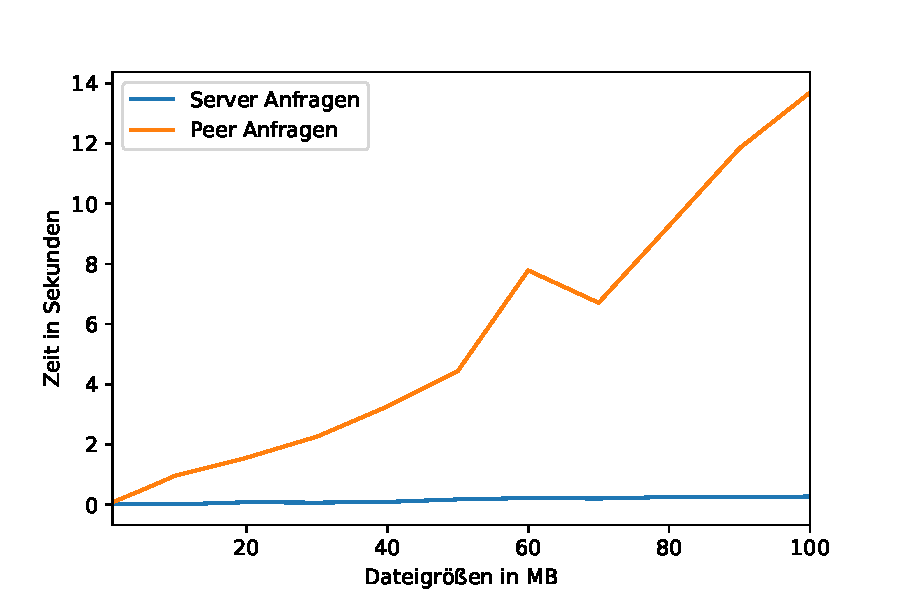
\includegraphics[width=0.8\textwidth]{figures/Timing_file_size}
	\caption[A Figure Short-Title]{Vergleich verschiedener Dateigrößen}
	\label{fig:timing_file_size}
\end{figure}

Um die Ladezeiten verschiedener Dateigrößen zu evaluieren wurde auf einem Mac book pro Ende 2013 mit 2.3 GHz und 16GB Arbeitsspeicher getestet. 
Getestet wurde mit zwei Teilnehmern. Einer lud die Ressource vor und der zweite lud sie über das \pTp \cdn. Die Timeouts des \pTp \cdns wurden für diesen Test deaktiviert. Alle tests wurden zehn Mal ausgeführt. Das \pTp Datenpackete wurden über das lokale Netzwerk geleitet.

\begin{figure}[!h]
	\centering
	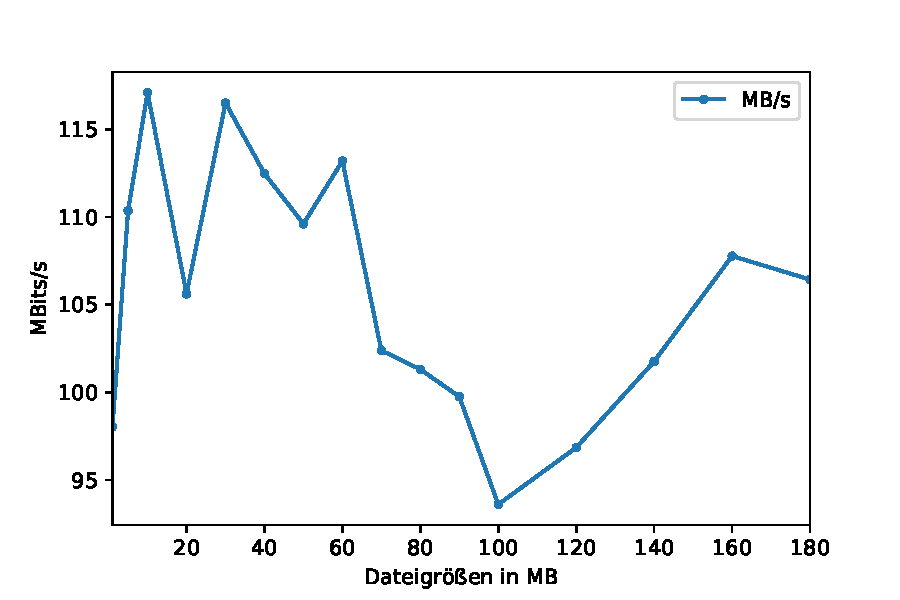
\includegraphics[width=0.8\textwidth]{figures/durchsatz_file_size}
	\caption[A Figure Short-Title]{Durchsatz des \ptp \cdns in einem lokalen Netzwerk}
	\label{fig:durchsatz_file_size}
\end{figure}

Abbildung \ref{fig:timing_file_size} zeigt wie sich das \cdn bei steigender Dateigröße verhält. Es ist deutlich zu sehen das die Ladezeit bei steigender Größe linear steigt. Zwar schwankt der Durchsatz des \cdns in einem Bereich von 20 MBits/s jedoch scheint es keinen Zusammenhang mit der Größe der Datei zu geben. Das Chunking der Dateien durch das \pTp \cdn scheint keinen negativen Einfluss auf die Ladegeschwindigkeit zu haben. Im Bereich von 100 MBits/s ist nach wie vor die zur Verfügung stehende Bandbreite und nicht das Chunking als Bottleneck zu betrachten.


%\begin{itemize}
%	\item Mac book pro Ende 2013
%	\item 2.3 ghz i7
%	\item 16gb ram
%	\item 1, 5, 10, 20, 30, 40, 50, 60, 70, 80, 90 , 100 mb
%	\item durchsatz berechnen
%	\item Limitierung durch websockets
%	\item lokal auf einem Rechner um Netzlaufzeiten auszuklammern
%	\item 1 Peer lädt vor
%	\item der andere lädt von peer
%	\item benchmarkt das nur das lokale netzwerk?? --> routing
%	\item sicherstellen das datenverkehr nicht über internet geroutet werden...
%\end{itemize}

\subsection{Live Streaming}
Um einen Live Stream mit höherer Teilnehmerzahl zu testen wurde ein Script geschrieben, das mit Hilfe von puppeteer\footnote{https://github.com/GoogleChrome/puppeteer} mehrere Chrome browser um headless Mode startet und die Event Seite besucht. Dabei musste eine Chrome installation gewählt werden, da Chromium nicht über die notwendigen Codecs verfügt um HLS Video wieder zu geben. 
Das Script wurde auf Amazon AWS t2.xlarge Instanzen installiert. Jede dieser Instanzen verfügt über 8 vcpus und 32 GB Arbeitsspeicher. Auf jeder Instanz wurden 25 Browser Sessions geöffnet.  Das \cdn wurde so konfiguriert das es ausschließlich .ts Dateien, also die Video Segmente bearbeitet. Bei 25 Teilnehmern lag die CPU Last bei den Testservern bei deaktiviertem \pTp \cdn bei 50-60\%. 
Die Teilnehmer luden die Event Seite während das Event noch nicht Live geschaltet war. Wenn alle Teilnehmer die Seite geladen hatten wurde das Event live geschaltet und die Teilnehmer auf die Live stream Seite weiter geleitet. Die Weiterleitung geschieht verzögert in einem Zeitraum von 18-60 Sekunden mit einer Dreicks-verteilung um die Last auf Seiten der Slidesync Servern zu verringern Der Stream wurde für zehn Minuten live geschaltet und anschließend beendet.

\begin{figure}[!h]
	\centering
	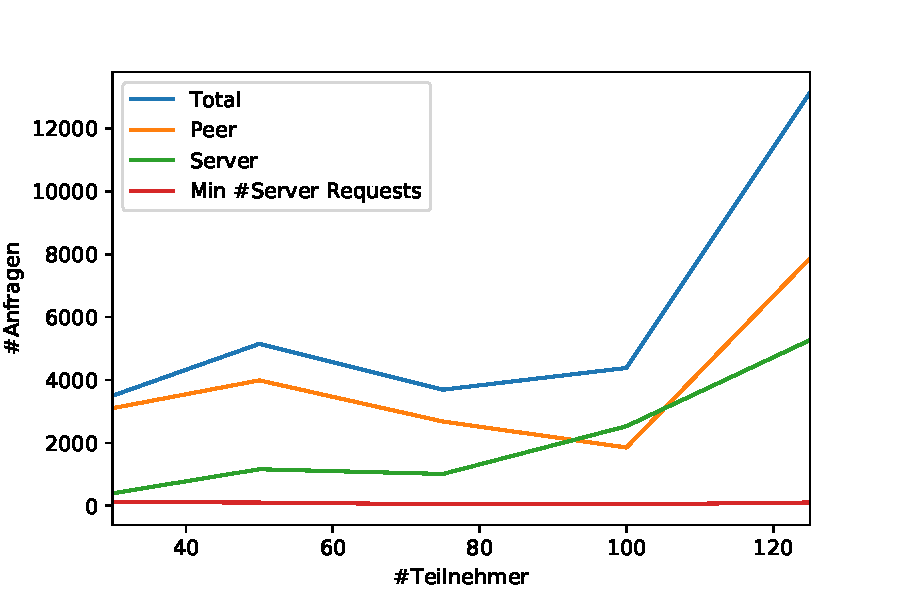
\includegraphics[width=0.8\textwidth]{figures/single_mesh_line}
	\caption[A Figure Short-Title]{Vergleich der Bearbeitung nach Art in einem Mesh}
	\label{fig:single_mesh_line}
\end{figure}

Abbildung \ref{fig:single_mesh_line} zeigt die wie sich das \pTp \cdn bei steigender Teilnehmerzahl mit einem Mesh verhält. Bis 50 Teilnehmern hat das \cdn ein lineares Verhalten hinsichtlich bearbeiteter Anfragen. Ab 75 Teilnehmern ist zu sehen das die Gesamtanzahl der verarbeiten Anfragen einbricht. Die CPU Last der Test Server stieg auf 100\% und die Clients waren dadurch nicht mehr in der Lage an dem \cdn Teilzunehmen und Anfragen zu bearbeiten. Der Kommunikationsaufwand die Peers in dem Mesh über Veränderungen des Caches zu Benachrichtigen wurde zu groß. Zwar wurden bei 125 Teilnehmern wieder mehr Anfragen vom \cdn verarbeitet, jedoch stieg der Anteil der Anfragen die über den Server liefen weiter an. Die höhere Anzahl an Anfragen die vom \cdn bearbeitet wurden ist vor allem darauf zurück zu führen, dass die Verbindungen zwischen den Peer durch die hohe Last teilweise unterbrochen wurde, wodurch sich die Last bei den Teilnehmern verringerte.   

\begin{figure}[!h]
	\centering
	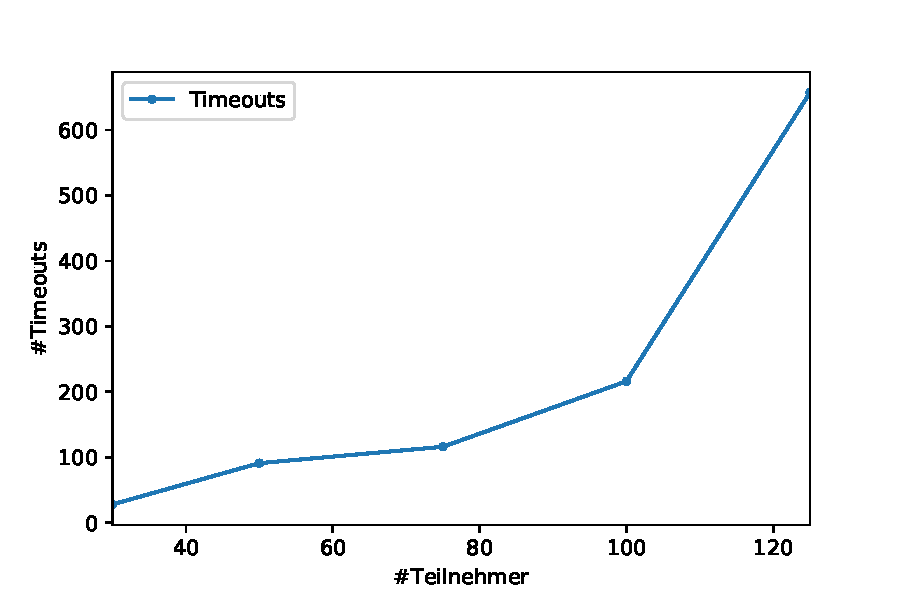
\includegraphics[width=0.8\textwidth]{figures/timeouts_single}
	\caption[A Figure Short-Title]{Timeouts bei einem Mesh}
	\label{fig:timeouts_single}
\end{figure}

Betrachtet man die Anzahl an Timeouts, so bestätigen sich die vorherigen Beobachtungen. Ab 75 Teilnehmern steigt die Anzahl an Timeouts stark an. Die CPU Last auf Seiten der Teilnehmern wurde zu groß um alle Anfragen in der geforderten Zeit zu beantworten. Neben der zu hohen Last ist kann es zu Timouts kommen falls zu viele Teilnehmer gleichzeitig eine Anfrage an den Selben Teilnehmer stellen. Der betroffene Teilnehmer ist in diesem Fall nicht in der Lage alle Anfragen schnell genug zu bearbeiten. Der Timeout wurde mit drei Sekunden so gewählt das es trotz Timeouts nicht zu einer Unterbrechung des Streams kommt. Der Video Player von Slidesync lädt drei HLS vor die je sechs Sekunden Video beinhalten insgesamt werden also 18 Sekunden vor geladen. Zu einer Unterbrechung der Wiedergabe kann es also erst kommen wenn eine Anfrage länger als 6 Sekunden benötigt. Da die längste verarbeitete Anfrage XXX Sekunden benötigte kam es zu keiner Unterbrechung der Wiedergabe aufgrund von Timeouts.

\begin{figure}[!h]
	\centering
	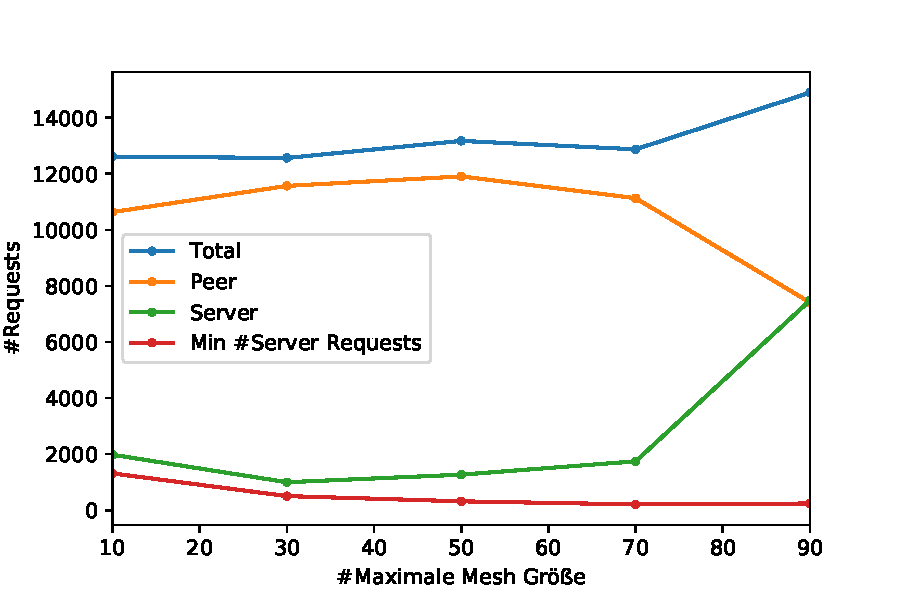
\includegraphics[width=0.8\textwidth]{figures/mesh_comparison}
	\caption[A Figure Short-Title]{Vergleich verschiedener Mesh Größen}
	\label{fig:mesh_comparison}
\end{figure}

\begin{figure}[!h]
	\centering
	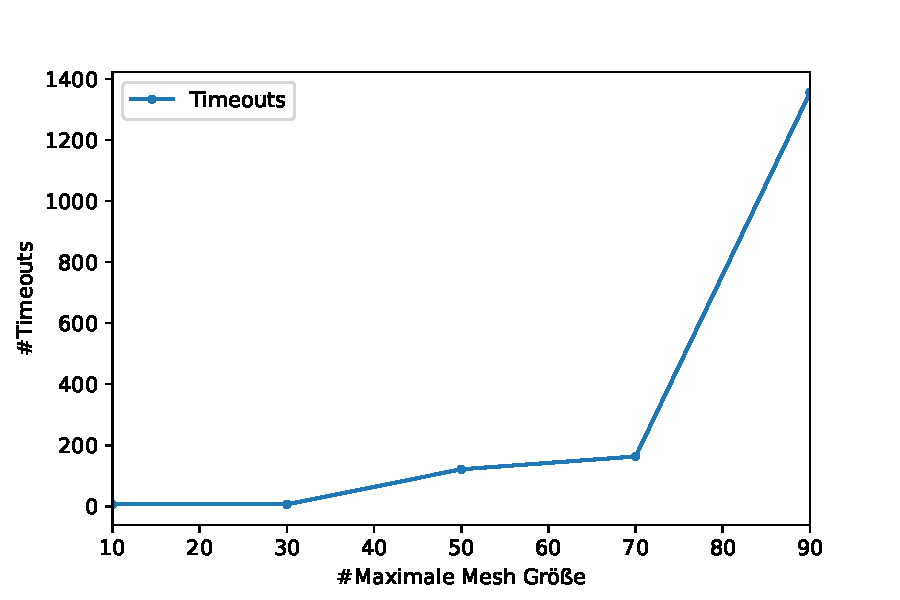
\includegraphics[width=0.8\textwidth]{figures/timeouts_meshed}
	\caption[A Figure Short-Title]{#Timeouts bei verschiedenen Mesh Größen (125 Teilnehmer)}
	\label{fig:timeouts_meshed}
\end{figure}

Abbildung \ref{fig:mesh_comparison} zeigt die Verarbeitungsart der Anfragen bei steigender Mesh Größe. Alle Tests wurden mit einer Teilnehmerzahl von 125 durchgeführt. Bei einer Mesh Größe von zehn ist die mindestanzahl an Anfragen die von dem Server beantwortet werden müssen mit 10\% relativ groß. Auch wenn nur selten Timeouts durch zu viele Anfragen bei dem selben Teilnehmer vorkommen konnten nur 84\% der Anfragen über das \pTp \cdn beantwortet werden. Die Beste Abdeckung hatte das \cdn bei einer Mesh Größe von 30 Teilnehmern mit 92\%. Bei einer Mesh Größe sind müssen mindestens 4\% der Anfrage über den Server beantwortet werden, damit jedes HLS Segment in jedem Peer Mesh vorhanden ist. Wird eine größere Mesh Größe als 30 gewählt so steigt auch die Anzahl der Timeouts ebenso wie die CPU Auslastung bei den Teilnehmern. So konnte bei einer Mesh Größe von 90 lediglich die Hälfte aller Anfragen durch das \pTp \cdn beantwortet werden.


\begin{figure}[!h]
	\centering
	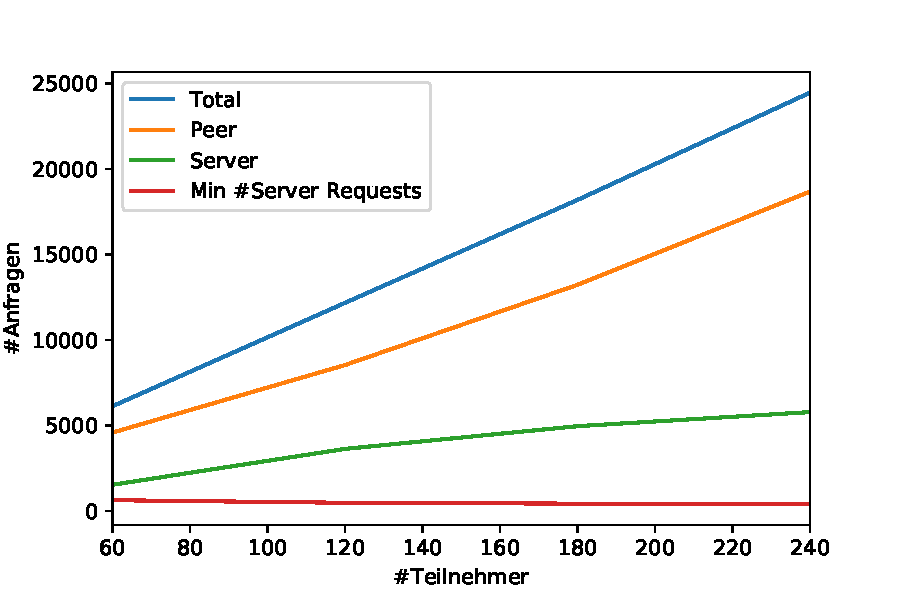
\includegraphics[width=0.8\textwidth]{figures/meshed_30_line}
	\caption[A Figure Short-Title]{Mesh Größe von 30 bei steigender Teilnehmer Zahl}
	\label{fig:meshed_30_line}
\end{figure}

Um zu testen wie sich das \cdn bei größeren Teilnehmerzahlen verhält wurden Tests mit einer Mesh Größe von 30 durchgeführt. Abbildung \ref{fig:meshed_30_line} zeigt einen Vergleich der Verarbeitungsarten. Die Anzahl an Peer Anfragen Verhält sich linear mit steigender Teilnehmerzahl. Die Abdeckung durch das \cdn schwankt zwischen 70-76\%.


\begin{figure}[!h]
	\centering
	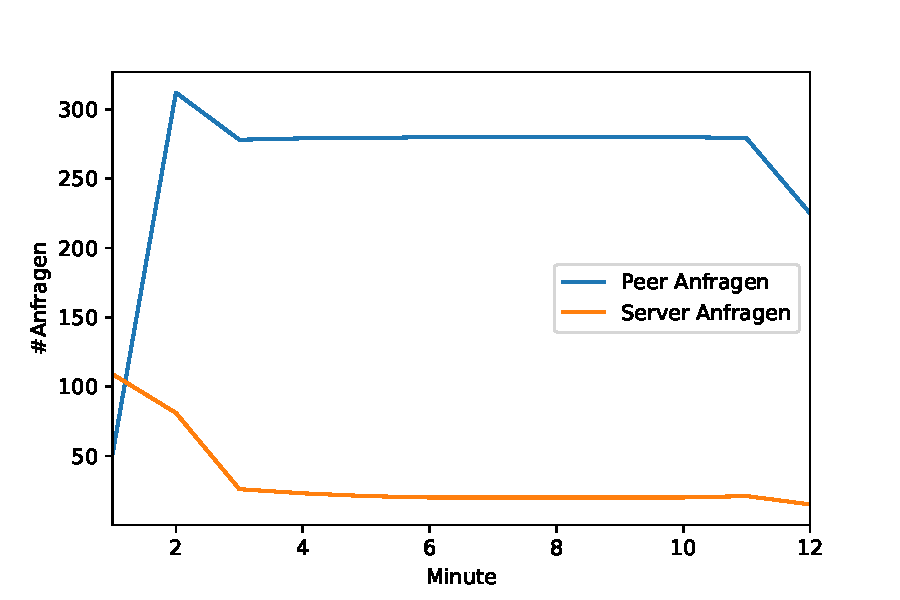
\includegraphics[width=0.8\textwidth]{figures/peer_vs_server_over_time}
	\caption[A Figure Short-Title]{Anfrageart über die Zeit bei 30 Teilnehmern}
	\label{fig:peer_vs_server_over_time}
\end{figure}

Abbildung \ref{fig:peer_vs_server_over_time} zeigt eine zeitliche Darstellung von beginn des Streams bis zum Ende des Streams für 30 Teilnehmer in einem Mesh. Es ist gut zu sehen, dass zu Beginn des Tests mehr Anfragen über die Server beantwortet werden müssen. Auch die Gesamtanzahl der Anfragen ist zu beginn des Tests höher als im späteren Verlauf. Nachdem die Seite geladen ist laden alle Teilnehmer drei HLS Segemente vor. Diese HLS Segmente werden gleichzeitig geladen, wodurch sich die Wahrscheinlichkeit erhöht das mehere Teilnehmer annähernd gleichzeitig die selbe Ressource anfragen und kein anderer Teilnehmer sie bereits geladen hat. 

%\begin{itemize}
%	\item Verhältnisse berechnen
%	\item evtl ramp up anschauen
%	\item  
%\end{itemize}

%\begin{itemize}
%	\item 92872 pro segment (ca 92 kb) 
%	\item ca 9,2 mb pro client pro event
%	\item bandbreiten diagram? 
%	\item Wenn client von server lädt teilt er das direkt mit
%\end{itemize}

\subsection{Schul-Cloud}
\begin{figure}[!h]
	\centering
	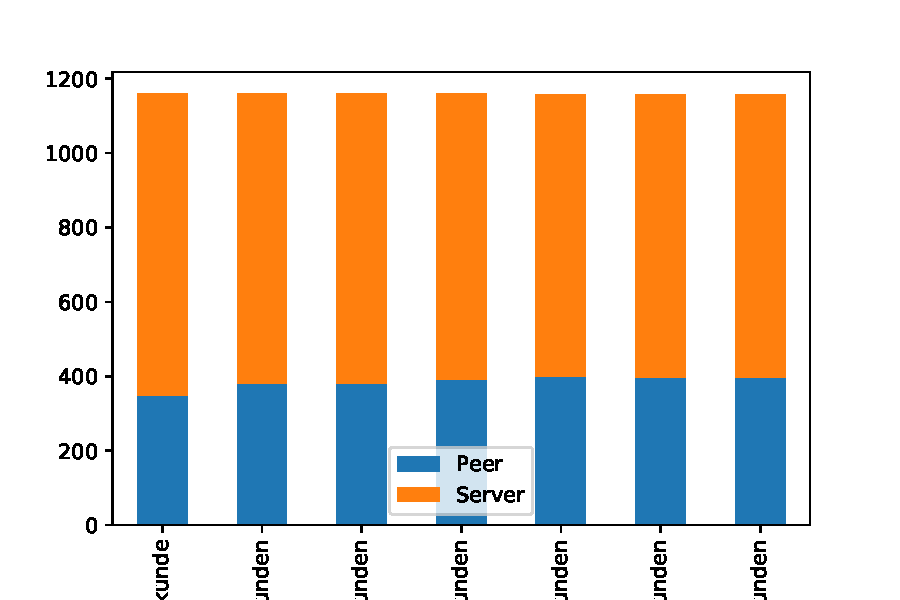
\includegraphics[width=0.8\textwidth]{figures/sc_stacked_interval}
	\caption[A Figure Short-Title]{Anfragearten gegliedert nach Ladeintervall}
	\label{fig:sc_stacked_interval}
\end{figure}
Um die Verwendung des \cdns in Schulen zu evaluieren wurde simuliert das 30 Schüler im Rahmen des Unterrichts auf die Seite Dashboard Seite zugreifen, die Kurs Liste Aufrufe einen Kurs Öffnen und ein Thema auswählen. Alle Clients wurden von einem Server aus gestartet und riefen die Seite zu einem zufälligen Zeitpunkt innerhalb verschiedener Intervalle auf. 

\begin{figure}[!h]
	\centering
	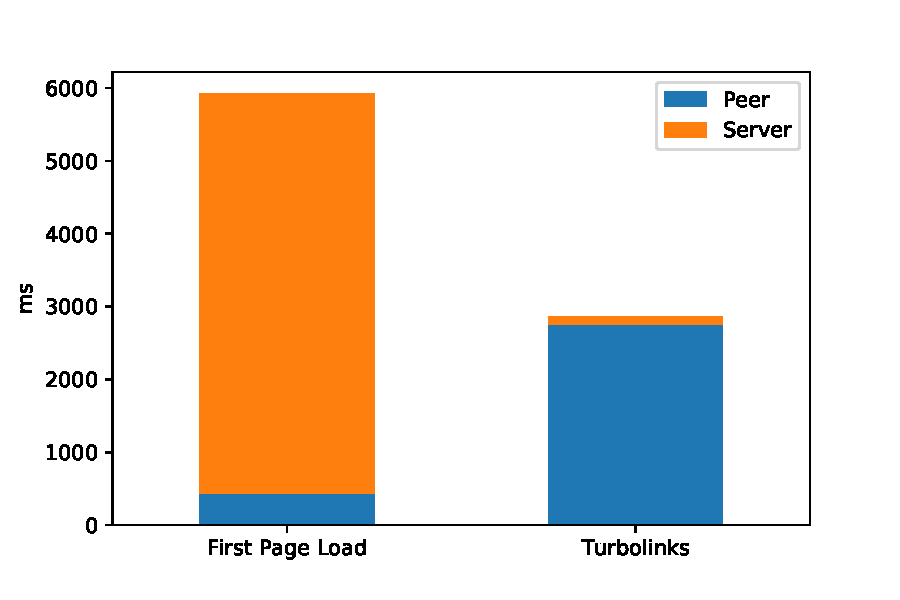
\includegraphics[width=0.8\textwidth]{figures/sc_first_vs_later}
	\caption[A Figure Short-Title]{Erstmaliges Laden vs. Navigation}
	\label{fig:sc_first_vs_later}
\end{figure}
Abbildung \ref{fig:sc_stacked_interval} zeigt die Verteilung der Anfragen nach Anfrage Art. Es ist gut zu sehen das die größe des Intervalls indem die Schüler auf die Seiten zugriffen keinen großen Einfluss auf die Effektivität des \pTp \cdns hatte. Zwar war die Effektivität bei einem Zugriff aller Schüler innerhalb einer Sekunde geringfügig schlechter, jedoch fällt dies kaum ins Gewicht. Bei einem Intervall von mehr als 5 Sekunden ist kaum noch eine Verbesserung der Effektivität zu beobachten.
\begin{figure}[!h]
	\centering
	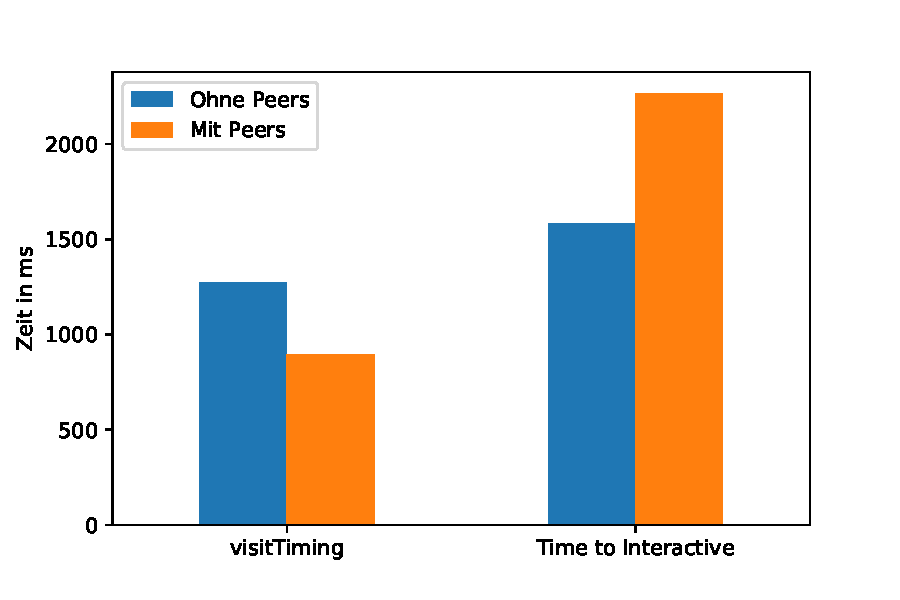
\includegraphics[width=0.8\textwidth]{figures/page_load_sc}
	\caption[A Figure Short-Title]{Seitenladezeiten}
	\label{fig:page_load_sc}
\end{figure}

Jedoch ist die Effektivität des \cdns bei den durchgeführten Tests bei nur ca. 38\%. Betrachtet man den Vergleich von dem ersten Laden der Seite und den folgenden Navigationen wird schnell ersichtlich worauf dies zurück zu führen ist. Beim ersten laden der Seite, einem kompletten Page Load, werden Anteilig deutlich mehr Anfragen gestellt als bei den folgenden Navigationen. Da das \cdn jedoch noch nicht komplett geladen ist kann nur ein kleiner Anteil der Anfragen durch das \cdn beantwortet werden. Da die Navigationen über Turbolinks gehandhabt wurden war kein kompletter Page Load notwendig. Das \cdn war zwar von Beginn der Navigation an verfügbar, jedoch war Turbolinks in der Lage einen Großteil der Anfragen zu vermeiden, da es sich um Assets handelte die für beide Seiten gleich waren. Ein erneutes Laden dieser Ressourcen war demnach nicht notwendig. Bei den Navigationen konnte das \cdn eine Effektivität von annähernd 100\% erreichen. 

\begin{figure}[!h]
	\centering
	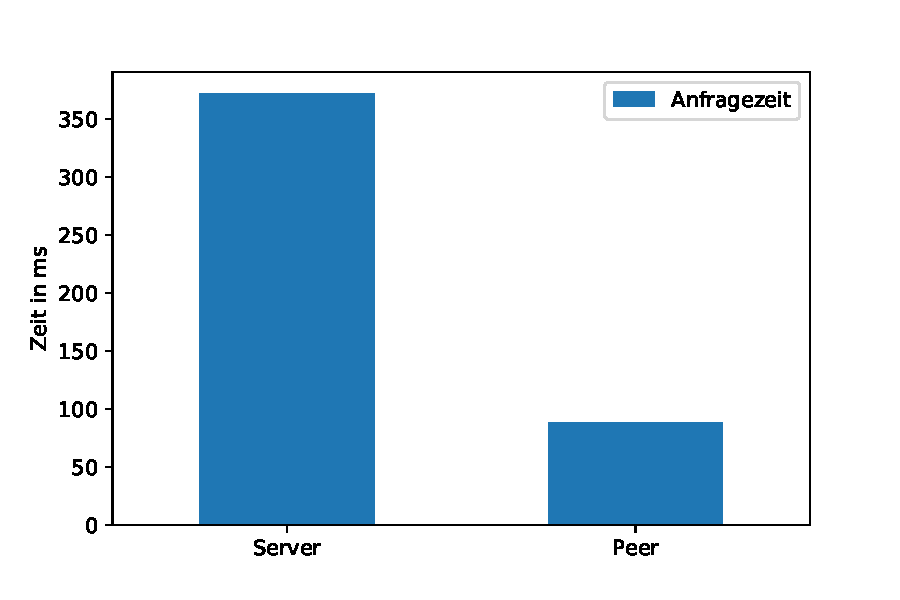
\includegraphics[width=0.8\textwidth]{figures/request_load}
	\caption[A Figure Short-Title]{Durchschnittliche Ladezeit von Anfragen nach Bearbeitungsart}
	\label{fig:request_load}
\end{figure}

Abbildung \ref{fig:page_load_sc} zeigt einen vergleich der Seitenladezeiten mit und ohne verfügbare Peers. Hierbei gilt zu beachten das für den ersten Page Load andere Metriken verwendet werden müssen als bei den Navigationen. Turbolinks greift in den Ladeprozess des Browsers ein wodurch Metriken die von den Browsern zur Verfügung gestellt werden, im Falle einer Navigation, incorrekte Daten zurück geben. Umgekehrt stellt Turbolinks zwar ebenfalls Methodiken zur Messung von Metriken bereit, jedoch geben diese für den ersten Page Load keine Ergebnisse zurück da Turbolinks diese Metriken selbst erfasst. Betrachtet man beide Fälle separat ist ein Vergleich jedoch möglich. Zur Messung des ersten Page Loads wurde die Time to Interactive gemessen. Es ist gut zu sehen das das \pTp \cdn einen gewissen Mehraufwand bedeutet. Bei den folgenden Navigationen kann jedoch eine Verbesserung der Ladezeit beobachtet werden. Dies ist vor allem auf die schnellere Beantwortung von Antworten zurückzuführen. Abbildung \ref{fig:request_load} zeigt deutlich das Anfragen die über das \pTp \cdn bearbeitet wurden deutlich schneller beantwortet werden konnten.
 

\section{Livestreaming in Unternehmensnetzwerken}
Um zu testen wie sich das \cdn innerhalb eines echten Netzwerks mit separaten Rechnern verhält wurde ein Livestream mit der Infrastruktur von Slidesync aufgesetzt. Slidesync verwendet bei der Verteilung des Videos das Datenformat HLS. Das \cdn wurde so konfiguriert das ausschließlich die HLS Segmente über das \cdn behandelt werden. Sämtliche im folgenden betrachteten Anfragen sind demnach HLS Segmente. 
\begin{figure}[!h]
	\centering
	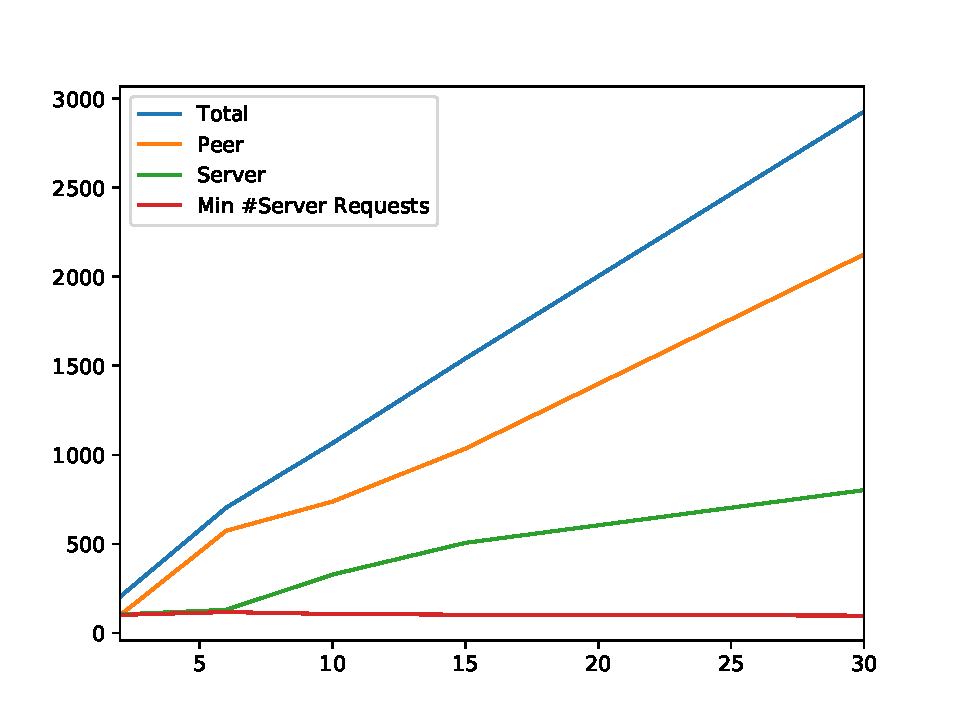
\includegraphics[width=0.8\textwidth]{figures/clients_line_chart}
	\caption[A Figure Short-Title]{Vergleich der Anfragen nach Anfrageart}
	\label{fig:live_stream_line_chart}
\end{figure}
Der Test wurde in einem Unternehmensnetzwerk durchgeführt um die Funktionalität in einem solchen Netzwerk zu gewährleisten. In diesem Netzwerk wurden insgesamt 30 Rechner aufgestellt. Da es vor allem um den Durchsatz des \cdns ging wurde auf allen Clients ein aktueller Chrome Browser verwendet. Auf den Clients wurde zuerst die Event Seite geladen und erst im Anschluss der Livestream gestartet. Getestet wurden sechs, zehn, 15, 20 und 30 Clients, die sich alle im selben lokalen Netzwerk befanden. Der Streaming- und der Anwendungsserver befand sich außerhalb des Netzwerkes und waren nur über die Internetverbindung zu erreichen. Bei jedem Test wurde der Stream zehn Minuten laufen gelassen und alle Clients befanden sich in dem selben Peer Mesh.

\begin{figure}[!h]
	\centering
	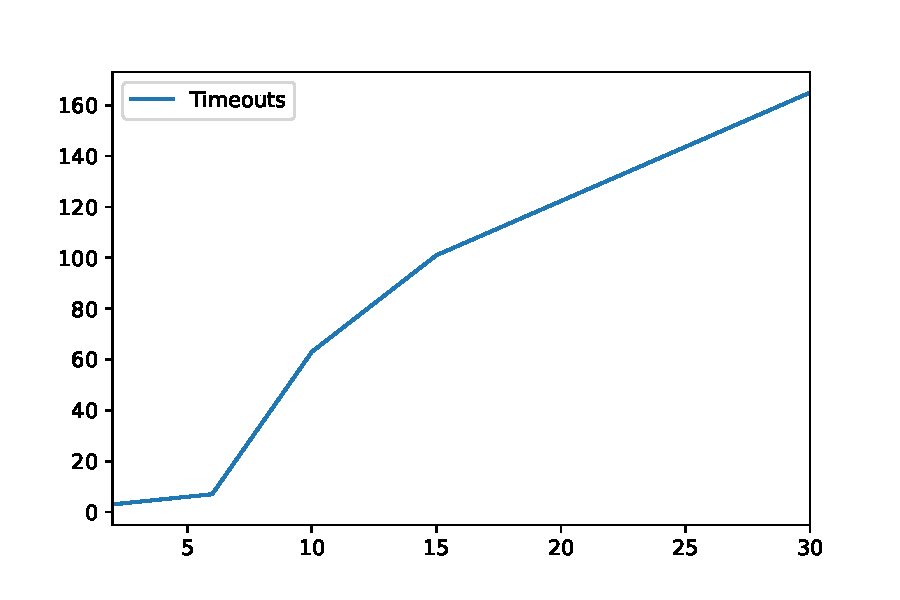
\includegraphics[width=0.8\textwidth]{figures/timeouts}
	\caption[A Figure Short-Title]{Anzahl der Timeouts des \cdns}
	\label{fig:timeouts}
\end{figure}


Abbildung \ref{fig:live_stream_line_chart} zeigt die Abhandlungsart der Anfragen. Dabei ist zu beachten das ca 100 Requests notwendig waren damit sämtliche HLS Segmente im \pTp Netzwerk verfügbar sind. Bei steigender Anzahl von Teilnehmern ist zu beobachten das eine größere Anzahl an Anfragen über den Server geladen werden müssen. Ein möglicher Grund hierfür ist Die Zeitliche Verteilung der Anfragen. Befinden sich mehr Peers im Netzwerk so wird es wahrscheinlicher das zwei Teilnehmer sich beide an der selben Stelle im Video befinden, die HLS Segmente laden müssen, jedoch noch kein Teilnehmer das Segment heruntergeladen hat. Auch wird es wahrscheinlicher das eine größere Anzahl an Teilnehmern ein Segment über den selben Teilnehmer laden wollen. Fragen zu viele Teilnehmer eine Ressource bei selben Teilnehmer an, so kann er nicht mehr alle Anfragen bearbeiten. Die Anfrage über das \pTp \cdn wird abgebrochen und über den Server geladen. Abbildung \ref{fig:timeouts} zeigt die Anzahl der Timeouts bei steigender Teilnehmerzahl. Dabei ist zu beachten das der Timeout so gewählt wurde das das Video weiterhin flüssig lief.


\begin{figure}[!h]
	\centering
	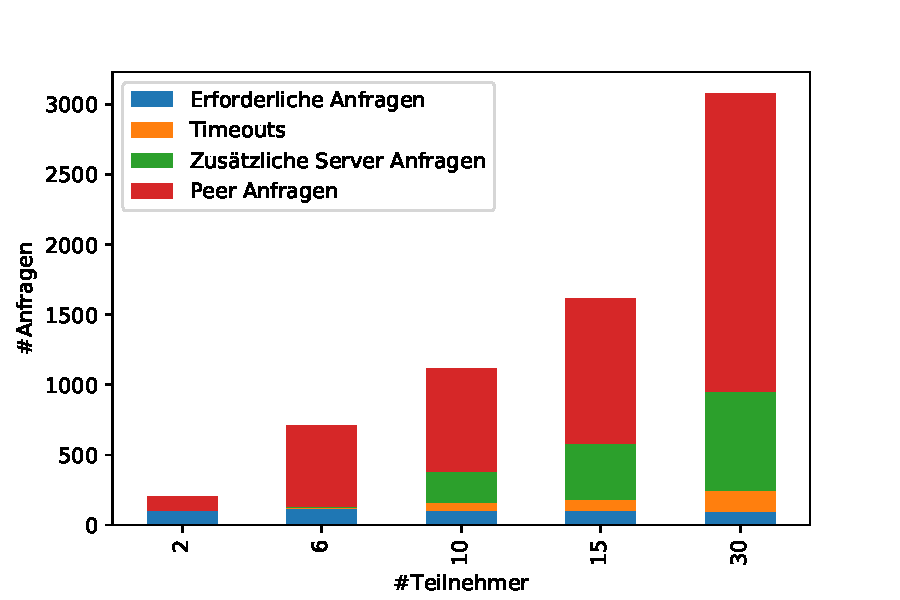
\includegraphics[width=0.8\textwidth]{figures/anfragen_verteilung_bar}
	\caption[A Figure Short-Title]{Vergleich der Anfragen nach Anfrageart}
	\label{fig:anfragen_verteilung_bar}
\end{figure}


Betrachtet man die zusätzlich notwendigen Server Anfragen so lässt sich beobachten das der Prozentsatz in diesem Test annähernd konstant ist.  

%\begin{figure}[!h]
%	\centering
%	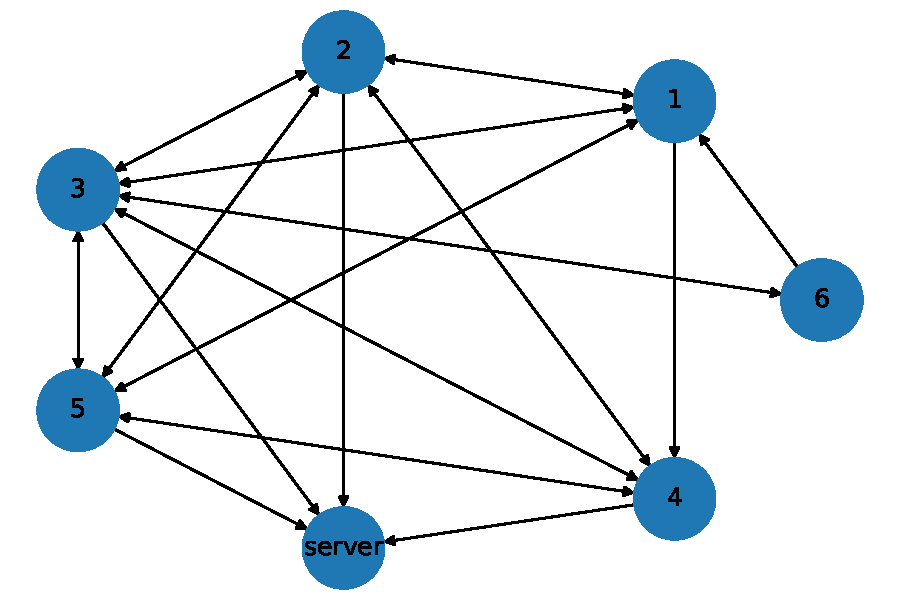
\includegraphics[width=0.8\textwidth]{figures/6_clients_network}
%	\caption[A Figure Short-Title]{Vergleich der Anfragen nach Anfrageart}
%	\label{fig:6_clients_network}
%\end{figure}

\begin{figure}[!h]
	\centering
	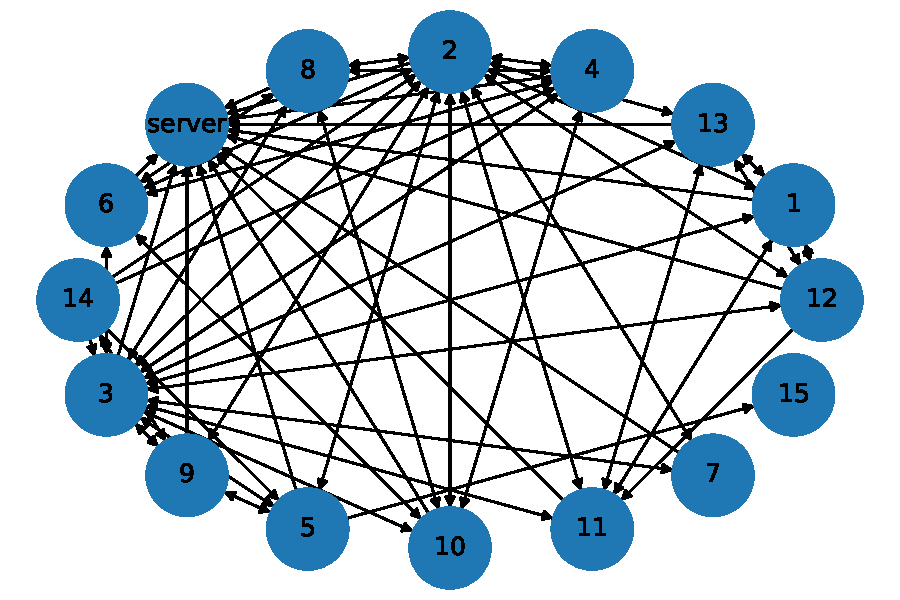
\includegraphics[width=0.8\textwidth]{figures/15_clients_network}
	\caption[A Figure Short-Title]{Vergleich der Anfragen nach Anfrageart}
	\label{fig:15_clients_network}
\end{figure}

Abbildung \ref{fig:15_clients_network} zeigt welche Teilnehmer untereinander Daten ausgetauscht haben. Auffällig ist das einige Teilnehmer besonders vielen Teilnehmern Daten gesendet haben. Dies war besonders dann der Fall wenn sie die einzigen im Netzwerk waren die das Segment bereits geladen hatten. Die meisten Kanten sind jedoch bidirektional, sprich zwar haben einige Teilnehmer besonders viele Anfragen beantwortet, jedoch haben sie sich nicht als zentrale Punkte des Netzwerkes etabliert sondern ebenfalls ihre Daten von anderen Teilnehmern geladen. \todo{gewichtung??} 

\begin{table}[!htb]
\begin{center}

	\begin{tabular}{|r|l|l|l|l|l|l|}
		\hline
		Bearbeitung	 & #Anfragen 	& Durchschnitt 	& Standardbweichung \\ \hline %	& Min		& Max	 \\ \hline
		Peer 		& 4571 				& 201.60	 ms	  	& 190.14	 ms	\\ \hline %			& 27.02 ms	& 2832.27 ms \\ \hline
		Server 		& 1870		 		& 63.61 ms		& 62.99	ms	\\ %			& 9.41 ms	& 649 ms	\\
		\hline
	\end{tabular}
	\caption{Verarbeitungsdauer}
\end{center}

\end{table}

Bei der Betrachtung der Ladezeiten wurden alle erfassten Anfragen berücksichtigt. Allerdings wurden die Daten um die Server Anfragen bereinigt bei denen zuvor das \pTp \cdn einen timeout verursacht hat. Insgesamt wurden 4571 Peer Anfragen und 1870 Server Anfragen betrachtet. 
Anfragen die vom \pTp \cdn beantwortet wurden brauchten im Durchschnitt 201,60ms. Server Anfragen waren im Vergleich mit 63,31ms im Durchschnitt deutlich schneller. Die ist auf den geringeren Durchsatz der \webrtc Datachannels zurückzuführen. (Siehe Dateigrößen \todo{ref}) Damit war das \pTp \cdn zwar deutlich langsamer, jedoch schnell genug um eine flüssige Wiedergabe zu gewährleisten. Da eine Anfrage die länger als 3000ms brauchte bei dem \pTp \cdn zu einem timeout geführt hat betrug die höchste erfasste Ladezeit 2832,27 ms.    
%\todo{einige clients haben keine daten an den server gesendet. Rausrechnen!}
%\begin{itemize}
%	\item ladezeiten
%	\item Alle Anfragen berücksichtigt
%	\item 4571.0 peerRequest
%	\item serverResponse   1870.0
%	\item Serveranfragen bereinigt um die Timeouts
%\end{itemize}
%\begin{itemize}
%	\item andere auflösungen
%	\item s vs p
%	\item server downloadtime berücksichtigen
%	\item besonders vergleich für hohe auflösungen
%	\item vergleich verschiedener Auflösungen
%\end{itemize}
%%passt hier nicht wirklich hin


\section{Offline Support}

Service Worker werden häufig im Rahmen von Offline-Support für Websites genannt. Mit Hilfe der Caching Api lassen sich Internetseiten speichern und später, wenn kein Internet vorhanden ist, wieder abrufen. Insbesondere für Schulen ist die Interessant, da die Internetanbindung in Schulen in vielen Fällen nach wie vor unzureichend ist. Die Sonderstudie Digital der Initiative befragte 2016 1426 Lehrer von denen 4\% Angaben das es an Ihrer Schule kein Internet gibt. In Rund 50\% der befragten Lehrer gab an das es Internet nur in bestimmten Räumen gebe.\cite{sonderstudie_digital} In Kombination mit einem \pTp \cdn lässt sich dies nutzen um Internetseiten und Ressourcen, auch im Falle eines Internetausfalls oder falls kein Internet vorhanden ist, zu laden. Insbesondere das Scenario das der Lehrer die Seite bzw. Inhalte zu Hause vor lädt und im Anschluss den Schülern bereit stellt erscheint interessant. Tobias Wollowski beschreibt in seiner Arbeit "Optimierung von Web-Anwendungen für den Einsatz im Klassenzimmer"\cite{tobi} Möglichkeiten zur Nutzung von Offline Caches im Unterricht. Im Folgenden wird Konzeptionell beschrieben wie das vorgestellte \pTp \cdn angepasst werden kann um auch im Falle einer nicht vorhandenen Internetanbindung funktionieren kann.

Durch die Verwendung von Service Workern als Proxy und Cache bietet das \cdn eine gute Grundlage für offline Support. Es stellt die Möglichkeit bereit Inhalte aus dem Cache an andere Nutzer zu verteilen. Die Größte Herausforderung bei der Offline Nutzung stellt das Signaling, also das Verbinden von Nutzern, dar. Um dies zu bewerkstelligen ist bei der gewählten Implementierung ein Websocket Server notwendig. Ist die Verbindung bereits hergestellt, z.B. vor einem Internetausfall, so können bereits bei der momentanenen Implementierung Inhalte in dem Peer Mesh verteilt werden. Ist dies nicht der Fall so muss im lokalen Netzwerk ein Signaling Server bereit gestellt werden, so das dieser auch ohne Internet Verbindung erreichbar ist. Auch muss der Schüler bestimmte Ressourcen wie das \pTp \cdn schon im Vorfeld geladen, und mit Hilfe eines Service Workers gespeichert, haben. Sind die Ips einiger Nutzer bereits bekannt, so ist es ebenfalls denkbar das weitere Signaling über Webrtc auszuhandeln. Dazu ließen sich Algorithmen wie Kademlia\cte{kademlia} zum auffinden von Peers verwenden. Der Größe Nachteil ist jedoch das initial die IP Adressen von Nutzern bekannt sein muss. Hassan Ijaz\cite{signaling_no_i_patent} beschreibt in verschieden Möglichkeiten um \webrtc Verbindungen auch ohne Internet aufzubauen. Unter anderem ist es möglich \webrtc Verbindungen mit Hilfe von QR Codes zu initialisieren. Der Lehrer könnte den Schülern einen QR code, oder in einer anderen Codierung, ein SDP Packet bereitstellen mit dessen Hilfe die Schüler eine \webrtc Verbindung zum Lehrer herstellen können. Anschließend fungiert der Lehrer als Signaling Server für die Schüler über \webrtc, so das Verbindungen zwischen den Schülern hergestellt werden können.

Offline Support ist für Livestreams vor allem Interessant um die Ausfallsicherheit zu erhöhen. Slidesync lädt 18 Sekunden Video vor bevor es abgespielt wird. Durch Verwendung des \pTp \cdn können kürzere Ausfälle überbrückt werden, so das zumindest ein Teil der Nutzer weiterhin das Video über andere Nutzer Laden und verteilen können. Ein Signaling ist nicht notwendig da die Verbindungen bereits hergestellt wurden. Da Unternehmen in aller Regel über ausreichende Internetverbindungen Verfügen und es sich um Live Inhalte handelt ist ein reiner Offline Support eher von geringem Interesse. 

%\begin{itemize}
%	\item Motivation: Internet in Schulen ist nicht immer verfügbar
%	\item lehrer lädt inhalte zuhause vor
%	\item stellt sie schülern zur Verfügung
%	\item wie funktionieren offline webanwendungen
%	\item Service Worker
%	\item prefetching
%	\item Live Streams: Ausfallsicherheit wird erhöht.
%	\item quasi bei design
%	\item Resourcen werden gecached und sind offline verfügbar
%	\item Tobias arbeit Refernzieren
%	\item Übertragung im lokalen Netzwerk möglich wenn verbindung aufgebaut ist
%	\item Signaling müsste in lokalem netzwerk sein z.b. Rechner vom Lehrer
%	\item signaling könnte über webrtc erfolgen z.b. über 
%	\item kademlia routing indem Peers als vermittler fungieren
%	\item 	evt. browser plugin
%	\item 	Wie das routing machen?
%	\item Offline scenario:
%	\item 	Lehrer Lädt ressourcen vor und macht sie für schüler verfügbar
%	\item 	Kein Internet vorhanden
%	\item 	Schüler laden Ressourcen von Lehrer
%\end{itemize}

\section{Sicherheit}
Bei der Verwendung von \pTp \cdns bringen einige Security Herausforderungen mit sich. Da dies nicht Schwerpunkt der Untersuchungen im Rahmen dieser Arbeit ist wird eine vertrauenswürdige Umgebung angenommen. Dennoch werden im Folgenden Herausforderungen im Bereich der Sicherheit bei der Verwendung eines \pTp \cdns beleuchtet und mögliche Lösungen vorgestellt.

Eines der Grundprinzipien des Internet Sicherheits Models ist das Nutzer bedenkenlos Internet Seiten aufrufen und dort Scripts laden können.\cite{huang_chen} Dieses Versprechen an den Nutzer muss der Browser garantieren um eine sichere Benutzung des Internet zu gewährleisten. Dazu werden Scripts in Sandboxes ausgeführt.\cite{chrome_sandbox} Ein Script kann nur im Kontext der aktuellen Seite ausgeführt werden und Anfragen die über die aktuelle Seite hinausgehen müssen vom Quellen Server explizit dafür frei gegeben werden.\cite{cors_std} 

Service Worker arbeiten nach dem Selben Prinzip. Sie haben keinen Zugriff auf das DOM und können nur Anfragen verarbeiten die unterhalb des Ihnen zugewiesenen Scopes, der Seite die sie geladen hat, liegen.\cite{moz_sw} Anfragen die über einen Service Worker behandelt werden und nicht der Same-Origin Policy folgen müssen mit dem Entsprechenden CORS Header versehen sein um geladen zu werden. Service Worker können nur über HTTPS geladen werden. Wird eine Ressource neu vom Server in das \pTp \cdn geladen so muss sie den gleichen Sicherheitsvorkehrungen des Browsers entsprechen wie jede andere Anfrage. Wird eine Anfrage über das \pTp \cdn selbst beantwortet so greifen diese Mechanismen jedoch nicht. Es ist möglich das ein bösartiger Client eine Ressource verändert bevor er sie an einen Client sendet, der diese dann lädt. 

Um die Integrität einer Ressource stellen Browser Funktionalitäten bereit die auf Hashes der Ressource beruhen die bei Anfrage mitgesendet werden.\cite{sub_res_integrity} Dies wird bei Anfragen automatisch durch den Browser übernommen. Bei der Übertragung mittels \webrtc muss dies die Anwendung selbst übernehmen.  

Durch die Verwendung von nativen Browser Funktionalitäten entfällt die Installation von Plugins oder Anwendungen. Dadurch entfällt das Risiko von Malware in Installationsdateien. Umso wichtiger ist jedoch das ein Vertrauenswürdiger Browser verwendet wird. Wurde der Browser aus einer unsicheren Quelle geladen, so kann eine sichere Verwendung des \cdns nicht gewährleistet werden, da die Sicherheitskonzepte auf der Implementation des Browser beruhen.\cite{webrtc-security}

Wird HTTPS bei der zugrundeliegenden Anwendung verwendet, so wird auch der Datenverkehr über Webrtc mittels TLS verschlüsselt.\cite{rtcweb-security} Daten die mittels \webrtc Datachannels gesendet werden, werden über DTLS(Datagram Transport Layer Security) übertragen. Dies geschieht auch falls ein TURN Server verwendet wird. Dadurch sind die Verbindungen Ende-zu-Ende verschlüsselt.

Die Websocket Verbindung die für das Signaling verwendet wird sollte ebenfalls verschlüsselt werden. Die Anwendung muss außerdem Sicherstellen, dass sich keine Clients, die nicht autorisiert sind mit sich deinem Websocket Channel verbinden, da sie ansonsten in der Lage sind Ressourcen anzufragen für die sie keine Berechtigung haben, oder schadhafte Scripts an Nutzer senden könnten.

\begin{figure}[!h]
	\centering
	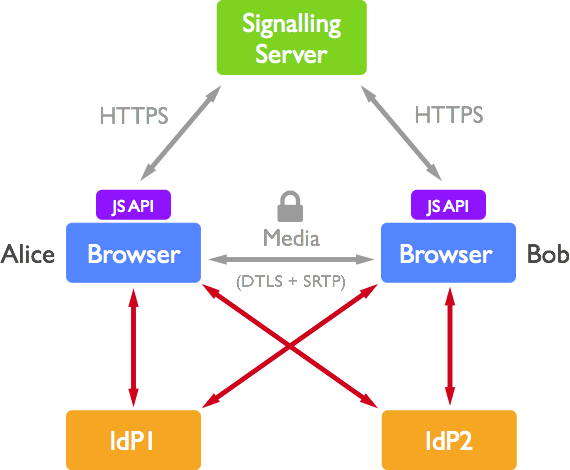
\includegraphics[width=0.8\textwidth]{figures/user_auth}
	\caption[A Figure Short-Title]{IdP basierter Verbindungsaufbau\cite{rtcweb-security}}
	\label{fig:user_auth}
\end{figure}

Ein weiteres in dem Schul Kontext zu betrachtendes Szenario ist die Verwendung eines Rechners von mehreren Nutzern. Viele Schulen haben Computerräume in denen Rechner stehen die von verschiedenen Klassen und Schülern verwendet werden. Zwar wäre es prinzipiell möglich den gesamten cache beim Login/logout zu löschen, jedoch würde das die Cache Trefferrate negativ beeinflussen. Um dies zu umgehen können die Ressourcen verschlüsselt gespeichert werden. Wird dazu ein Schlüssel verwendet der nur im aktuellen Scope verfügbar ist so kann er sie nur entschlüsselt werden falls der Nutzer Zugriff auf den Scope der Resource hat. Ein unbefugtes auslesen des Caches ist somit zwar möglich, jedoch sind die Daten für den Angreifer unbrauchbar.

Auch wenn der Signaling Server einen Teil der Nutzer Authentizität sicher stellt so sollte diesem nicht vollkommen vertraut werden. Der Signaling Server kann lediglich sicher stellen das ein Nutzer in eine bestimmte sicherheitsklasse gehört, da er nur den Zugriff auf einen Websocket Channel sicher stellt. Ist es darüber hinaus notwendig die Autentizität eines Nutzers zu gewährleisten können Web basierte Identitäts Provider(IdP) verwendet werden. Diese fungieren als vertrauenswürdige Partei und können die Identität eines Nutzers bestätigen. Abbildung \ref{fig:user_auth} zeigt die Struktur einer solchen Verbindung.

Durch die Verwendung von \webrtc, bei der Verwendung von STUN Servern besteht das Risiko eines IP-Leaks.\cite{rtcweb-security} Es ist prinzipiell möglich die IP-Adresse eines Nutzers zu ermitteln. Eine mögliche Gegenmaßnahmen ist die Deactivierung von Webrtc. Dies kann entweder in der Browser Konfiguration oder durch Plugins geschehen. Jedoch ist dann die Verwendung von \webrtc nicht mehr möglich. Um eine direkte Verbindung zu einem anderen Nutzer aufzubauen ist es notwendig dessen IP-Adresse zu ermitteln. Stellt die Gefahr eines IP-Leaks ein großes Risiko in der betrachteten Domäne da, so kann das \pTp \cdn nicht verwendet werden. Im Rahmen dieser Masterarbeit wird jedoch nur die Verbindung im Lokalen Netzwerk, ohne die Verwendung eines STUN Servers untersucht. Es besteht also lediglich die Gefahr das die lokale IP Adresse eines Nutzers ermittelt werden kann - Nicht jedoch dessen öffentlich IP Adresse.


%\begin{itemize}
%	\item http://www.adambarth.com/papers/2011/huang-chen-barth-rescorla-jackson.pdf [huang_chen]
%	\item https://blog.cryptographyengineering.com/2012/01/10/attack-of-week-datagram-tls/
%	\item https://tools.ietf.org/html/draft-ietf-rtcweb-security-05 [rtcweb-security]
%	\item ---
%	\item Vertrauensbeziehung zwischen Clients
%	\item Websocket channels müssen gesichert werden!
%	\item Trust enviroment
%	\item resource integrity
%	\item hash
%	\item in logik
%	\item 
%	\item dateien im local cache verschlüsseln nur entschlüsseln durch kurs
%	\item mehrere an einem Rechner
%\end{itemize}
%\begin{itemize}
%	\item Owasp
%%	\item https://www.owasp.org/images/9/90/OWASP_Top_10-2017_de_V1.0.pdf
%	\item IP Leak möglich
%	\item Stun Server kann nach IP Adresse fragen
%	\item Über js auslesbar
%	\item Pluckins können das blocken
%	\item media.peerconnection.enabled ausschalten
%	\item --> kein webrtc mehr möglich
%	\item non repudiation
%	\item accountability
%
%\end{itemize}

